%
% File: chap03-03-02.tex
% Author:
% Description:
% 3.3 Back-end Design & Implementation
%  3.3.2 Database Design
%     Entity Relationship Design
%     Database Schema Implementation
%     Data Security and Privacy Considerations
%

After we finished the detailed discussion of each page’s user flow, we moved on to database design. Our first task was to clarify what kinds of data the system must store, and map them to a clear set of entities and relationships. We first created a rough data model on dbdiagram.io /reference as a quick way to communicate and iterate. During modelling, we noticed several issues in button navigation and page flow. To avoid a mismatch between frontend and backend, we worked in parallel—“draw the diagram and verify the flow at the same time”—and actively met with teammates to unify the detailed flows and the data to read/write. After that, for every system button or operation, we traced back the required primary/foreign keys and necessary column types, and then integrated all of these needs into the final data model.

% 確保有載入:\usepackage{graphicx}



The system’s full relationship structure is shown with crow’s-foot notation /reference. We implemented the revised schema in MySQL and used DBeaver’s reverse engineering /reference to automatically generate the ERD from the live database. All ERDs in the final report were exported from DBeaver to ensure the diagrams match the actual tables, as shown in Figure~\ref{fig:final_erd}.

\begin{figure}[!htbp]
  \centering
  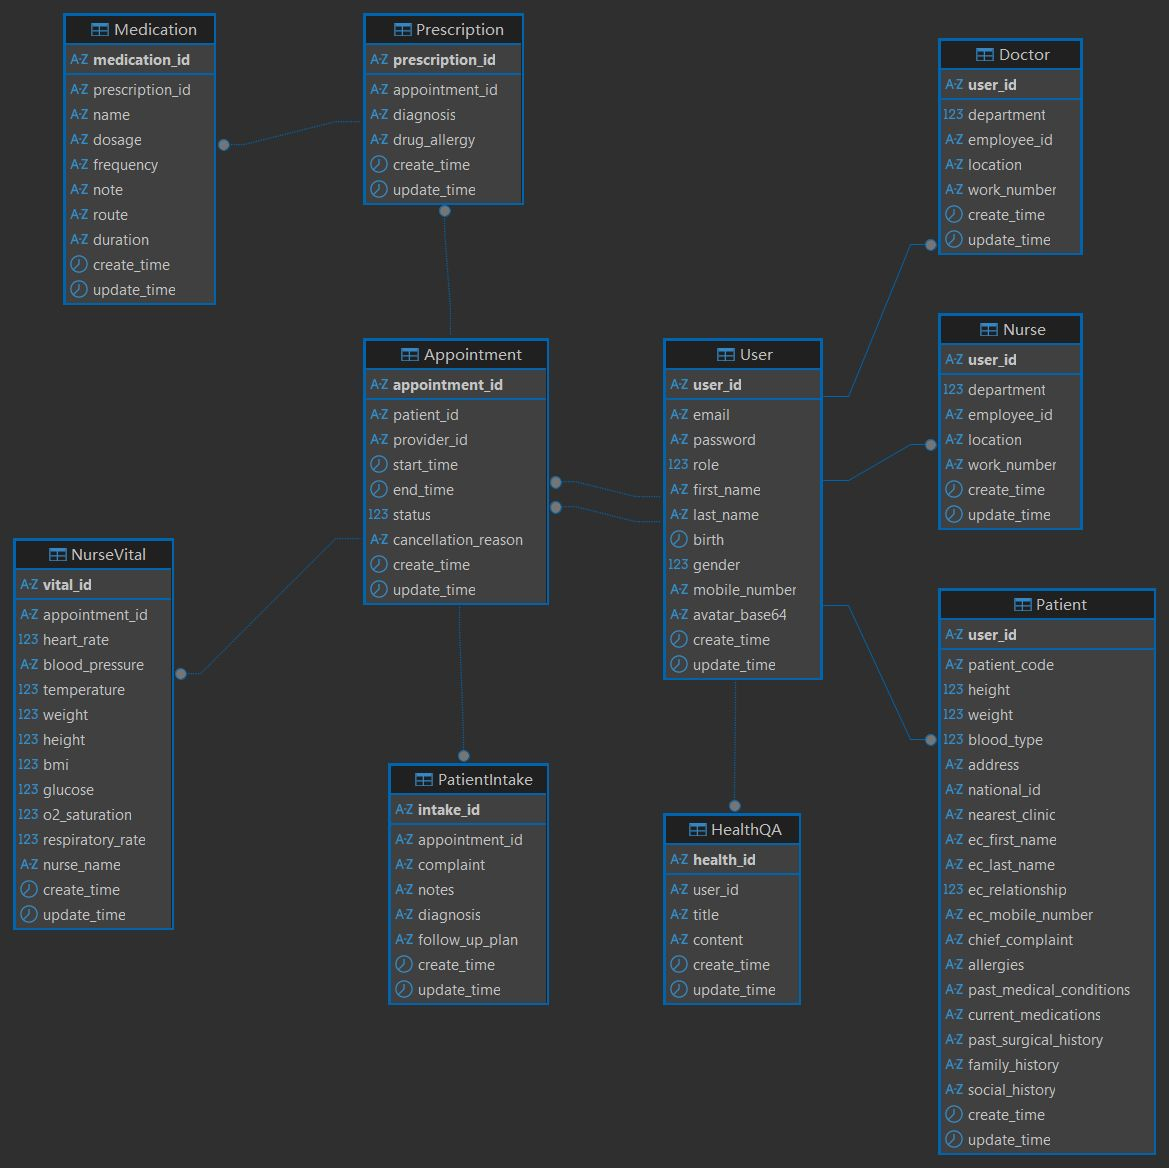
\includegraphics[width=\linewidth]{../../images/ERD.jpeg}
  \caption{Final ERD (reverse-generated from MySQL via DBeaver /reference).}
  \label{fig:final_erd}
\end{figure}
\FloatBarrier

From the figure, you can see an appointment-centred, single-visit data flow. \texttt{NurseVital} and \texttt{PatientIntake} (later renamed on the frontend to Clinical Note) correspond to nurse and doctor records. \texttt{Prescription} together with multiple \texttt{Medication} rows describes the treatment plan. For the HealthQA interaction, although we decided not to implement it due to time limits, we still designed the tables so it’s ready for future work. The column types and indexing plan (for example, a unique index on \texttt{User.email}, a composite index on \texttt{Appointment(patient\_id, provider\_id, start\_time)}, and indexes on all major foreign keys) are summarised in Appendix~Y.

Overall, this data model supports the core operations defined in our user flows (creating/cancelling appointments, recording vitals, filling consultation summaries, issuing prescriptions, and viewing medical history), while leaving space for extensions like report files and the Health Q\&A feature. It keeps the Smart Hospital system consistent and maintainable.
